\documentclass[11pt,a4paper,openany]{ctexrep}
\usepackage[a4paper,margin=23mm,headheight=15pt]{geometry}
\usepackage{amsmath,amssymb,mathtools,bm}
\usepackage{siunitx}
\usepackage{booktabs,tabularx,array,longtable}
\usepackage{enumitem}
\usepackage{graphicx}
\usepackage{xcolor}
\usepackage{tikz}
\usetikzlibrary{arrows.meta,positioning,shapes.geometric,calc,fit,decorations.pathmorphing}
\usepackage[most]{tcolorbox}
\usepackage{hyperref}
\usepackage{fancyhdr}
\usepackage{titlesec}
\usepackage{microtype}
\usepackage{setspace}

\definecolor{KidBlue}{HTML}{22577A}
\definecolor{KidTeal}{HTML}{2A9D8F}
\definecolor{KidGold}{HTML}{E9C46A}
\definecolor{KidRed}{HTML}{C8553D}
\definecolor{KidGray}{HTML}{F3F5F7}
\definecolor{KidDark}{HTML}{263238}

\hypersetup{colorlinks=true,linkcolor=KidBlue,urlcolor=KidBlue,citecolor=KidTeal,pdftitle={KID入门讲义 v0.1},pdfauthor={ChatGPT 辅助整理}}
\setstretch{1.15}
\setlist[itemize]{leftmargin=2em,itemsep=0.25em,topsep=0.4em}
\setlist[enumerate]{leftmargin=2em,itemsep=0.25em,topsep=0.4em}
\setlength{\parindent}{2em}
\setlength{\parskip}{0.25em}

\pagestyle{fancy}
\fancyhf{}
\fancyhead[L]{KID 入门讲义 v0.1}
\fancyhead[R]{\leftmark}
\fancyfoot[C]{\thepage}
\renewcommand{\headrulewidth}{0.4pt}

\titleformat{\chapter}[display]{\bfseries\Huge\color{KidDark}}{\filleft\color{KidBlue}\fontsize{44}{44}\selectfont\thechapter}{1ex}{\titlerule\vspace{1ex}\filright}
\titleformat{\section}{\Large\bfseries\color{KidBlue}}{\thesection}{0.7em}{}
\titleformat{\subsection}{\large\bfseries\color{KidTeal}}{\thesubsection}{0.7em}{}

\newtcolorbox{goalbox}{colback=KidBlue!5,colframe=KidBlue,boxrule=0.8pt,arc=2mm,title=本节目标,fonttitle=\bfseries}
\newtcolorbox{intuitionbox}{colback=KidTeal!6,colframe=KidTeal,boxrule=0.8pt,arc=2mm,title=物理直觉,fonttitle=\bfseries}
\newtcolorbox{projectbox}{colback=KidGold!16,colframe=KidGold!80!black,boxrule=0.8pt,arc=2mm,title=映射到你的 150 GHz LEKID,fonttitle=\bfseries}
\newtcolorbox{mistakebox}{colback=KidRed!5,colframe=KidRed,boxrule=0.8pt,arc=2mm,title=常见误区,fonttitle=\bfseries}
\newtcolorbox{checkpointbox}{colback=KidGray,colframe=KidDark!55,boxrule=0.7pt,arc=2mm,title=理解检查,fonttitle=\bfseries}
\newtcolorbox{formula}[1][]{colback=white,colframe=KidBlue!75,boxrule=0.9pt,arc=1mm,#1}

\newcommand{\qp}{\mathrm{qp}}
\newcommand{\Stwentyone}{S_{21}}
\newcommand{\fzero}{f_0}
\newcommand{\Qi}{Q_i}
\newcommand{\Qc}{Q_c}
\newcommand{\Qr}{Q_r}
\newcommand{\Lk}{L_k}
\newcommand{\Lg}{L_g}

\begin{document}

\begin{titlepage}
\centering
\vspace*{2.2cm}
{\fontsize{30}{38}\selectfont\bfseries\color{KidDark} KID 入门讲义}\par
\vspace{0.5cm}
{\Large\color{KidBlue} 从“一个光子”到可读出的微波信号}\par
\vspace{1.4cm}
{\large Version 0.1 · 2026-09-03}\par
\vfill
\begin{tcolorbox}[width=0.88\textwidth,colback=KidGray,colframe=KidBlue!55,arc=3mm]
\centering
\large
这不是一本“先学完凝聚态物理再碰器件”的教材。\\[0.5em]
它采用器件设计者视角：\\[0.3em]
\textbf{先建立可运行的物理图景，再逐层补上微观理论、公式、仿真与实验。}
\end{tcolorbox}
\vfill
{\large 面向：毫米/亚毫米波 KID / LEKID 初学与器件设计}\par
\end{titlepage}

\tableofcontents
\clearpage

\chapter*{如何使用这份讲义}
\addcontentsline{toc}{chapter}{如何使用这份讲义}
这份讲义按“\textbf{物理因果链}”而不是按学科目录组织。每一章都尽量回答四个问题：
\begin{enumerate}
  \item \textbf{发生了什么？} —— 先建立可视化的物理图景；
  \item \textbf{为什么？} —— 用最少但必要的公式把直觉固定下来；
  \item \textbf{怎么测？} —— 把物理量连接到真实实验中的 $I/Q$、$\Stwentyone$、频移和噪声；
  \item \textbf{与 LEKID 设计有什么关系？} —— 把材料、几何、电磁仿真和读出重新接回同一条链。
\end{enumerate}

当前版本 v0.1 重点完成两件事：
\begin{itemize}
  \item 给出整个 KID 入门学习路线；
  \item 完整建立第 1 章“从光子到 $\Stwentyone$”的基础物理图景。
\end{itemize}
后续版本会逐章增加推导、数值练习、Python notebook、Sonnet/全波仿真任务以及与你的双偏振 LEKID 项目的对应分析。

\chapter{KID 入门的总体路线图}

\section{最终要学会的不是一堆名词，而是一张闭环图}
对于一个真正能够设计、仿真和读出 KID 的研究者，知识最后应当闭合成下面这条链：

\begin{center}
\begin{tikzpicture}[node distance=6mm and 7mm, every node/.style={font=\small}, box/.style={draw,rounded corners,align=center,minimum height=10mm,fill=white}, arr/.style={-{Latex[length=2mm]},thick,KidBlue}]
\node[box,fill=KidGold!20] (opt) {入射光场\\$P_{\rm opt},\nu$};
\node[box,right=of opt] (pair) {超导微观态\\$\Delta,N_{\qp}$};
\node[box,right=of pair] (cond) {复电导\\$\sigma_1-i\sigma_2$};
\node[box,right=of cond] (res) {谐振器\\$f_0,Q_i$};
\node[box,below=of res] (s21) {微波读出\\$\Stwentyone=I+jQ$};
\node[box,left=of s21] (noise) {噪声与灵敏度\\NEP, TLS, GR};
\node[box,left=of noise] (em) {LEKID 电磁结构\\吸收/偏振/背短};
\draw[arr] (opt)--(pair);
\draw[arr] (pair)--(cond);
\draw[arr] (cond)--(res);
\draw[arr] (res)--(s21);
\draw[arr] (s21)--(noise);
\draw[arr] (em)--(noise);
\draw[arr] (opt) |- (em);
\end{tikzpicture}
\end{center}

你最终要能够在这张图中从任意一格走到任意一格。例如：
\begin{itemize}
  \item 改变膜厚，为什么会影响吸收、$\Lk$、$Q_i$ 和 responsivity？
  \item 加 backshort，为什么主要先改变毫米波吸收，却最终体现在 GHz 读出端的 $I/Q$ 上？
  \item 为什么同样一个 $\Stwentyone$ notch，可能对应完全不同的光学效率？
\end{itemize}

\section{建议的学习模块}
\renewcommand{\arraystretch}{1.25}
\begin{tabularx}{\textwidth}{>{\bfseries}p{1.5cm} p{4.0cm} X p{2.6cm}}
\toprule
模块 & 核心主题 & 学完后应该能回答的问题 & 典型产出 \\
\midrule
M1 & 从光子到 $\Stwentyone$ & KID 到底怎样把光变成可测的 IQ 变化？ & 因果链 + 极简仿真 \\
M2 & 超导基础 & Cooper pair、能隙、准粒子到底是什么？ & BCS 最小知识集 \\
M3 & 动能电感与复电导 & 为什么超导载流子的惯性等效为电感？$\sigma_1,\sigma_2$ 如何进入器件？ & $L_k$ 推导 + MB 框架 \\
M4 & 微波谐振器 & $Q_i,Q_c,Q_r$、耦合和 IQ 圆分别意味着什么？ & resonator fitting \\
M5 & 光学响应 & 光功率如何映射为 $\Delta f_0$、相位和幅度？ & responsivity 模型 \\
M6 & 噪声与 NEP & 什么时候是 photon-noise limited？TLS、GR、放大器噪声如何比较？ & noise budget \\
M7 & LEKID 电磁设计 & meander 为什么既是 absorber 又是 inductor？IDC、偏振、backshort 如何设计？ & 参数化像素模型 \\
M8 & 阵列与读出 & 如何频分复用数百/数千像素？tone spacing、动态范围如何约束设计？ & readout budget \\
M9 & 仿真与实验 & Sonnet/CST/测量数据各自验证哪一层物理？ & 仿真-测量闭环 \\
M10 & 研究课题化 & 如何从“能工作的 KID”走向可发表的问题？ & 论文问题与验证矩阵 \\
\bottomrule
\end{tabularx}

\section{推荐学习顺序}
不建议一上来死磕 Mattis--Bardeen 积分。更高效的顺序是：
\[
\boxed{
\text{可视化因果链}
\rightarrow
\text{等效电路}
\rightarrow
\text{最小超导理论}
\rightarrow
\text{复电导}
\rightarrow
\text{噪声与光学}
\rightarrow
\text{LEKID 工程设计}
}
\]
这使得每一个新公式都有“它为什么值得学”的位置。

\chapter{从一个光子到 $S_{21}$：KID 的第一性物理图景}

\begin{goalbox}
学完本章后，你应该能不看资料独立讲清：
\begin{enumerate}
  \item 为什么毫米波/亚毫米波光子能够改变超导薄膜；
  \item 为什么这种变化会改变 kinetic inductance 和 microwave loss；
  \item 为什么谐振频率与品质因数因此改变；
  \item 为什么实验最终读到的是 $\Stwentyone=I+jQ$；
  \item 一颗 LEKID 为什么可以同时扮演“光学吸收器”和“GHz 微波谐振器”。
\end{enumerate}
\end{goalbox}

\section{先看全局：KID 是一台“两种频率协同工作”的机器}
KID 初学时最容易混淆的一点，是把“被探测的光”和“用于读出的微波”混为一谈。事实上，它们通常相差几十到上百倍频率。

\begin{center}
\begin{tikzpicture}[node distance=7mm and 10mm, every node/.style={font=\small}, b/.style={draw,rounded corners,align=center,minimum height=11mm,minimum width=26mm}, a/.style={-{Latex[length=2.2mm]},very thick}]
\node[b,fill=KidGold!23] (ph) {信号光子\\例如 \SI{150}{GHz}};
\node[b,right=of ph,fill=KidGold!13] (film) {超导薄膜\\吸收能量};
\node[b,right=of film,fill=KidTeal!10] (qp) {$N_{\qp}\uparrow$\\超导态改变};
\node[b,right=of qp,fill=KidBlue!8] (res) {$L_k,Q_i$ 改变\\$f_0$ 移动};
\node[b,below=13mm of res,fill=KidBlue!8] (iq) {$\Stwentyone=I+jQ$\\随时间变化};
\node[b,left=of iq,fill=KidGray] (adc) {放大器/ADC\\数字读出};
\node[b,left=of adc,fill=KidGray] (probe) {探针微波\\例如 \SIrange{1}{5}{GHz}};
\draw[a,KidGold!80!black] (ph)--(film);
\draw[a,KidGold!80!black] (film)--(qp);
\draw[a,KidTeal] (qp)--(res);
\draw[a,KidBlue] (res)--(iq);
\draw[a,KidBlue] (iq)--(adc);
\draw[a,KidBlue] (probe)--(adc);
\draw[a,KidBlue,dashed] (probe) |- (res);
\end{tikzpicture}
\end{center}

一句话概括：
\begin{formula}
\[
\boxed{
P_{\rm opt}
\rightarrow N_{\qp}
\rightarrow (L_k,Q_i)
\rightarrow (f_0,Q_r)
\rightarrow S_{21}
\rightarrow I,Q
}
\]
\end{formula}

\begin{intuitionbox}
\textbf{信号光子负责“改变器件”，GHz 探针微波负责“询问器件”。}\\
KID 的巧妙之处，不是把毫米波直接送进 GHz ADC，而是让毫米波先改变一个非常灵敏的超导谐振器，再用微波精确测量这个变化。
\end{intuitionbox}

\section{第一站：入射光子必须有足够的能量}

\subsection{光子的能量尺度}
一个频率为 $\nu$ 的光子能量为
\[
E_\gamma=h\nu.
\]
对于 \SI{150}{GHz}：
\[
E_\gamma = h\nu \approx \SI{9.94e-23}{J}\approx \SI{0.620}{meV}.
\]
这个数本身没有意义，直到我们把它与超导体的能隙 $\Delta$ 比较。

\subsection{超导能隙与 pair-breaking threshold}
在弱耦合 BCS 近似下，零温能隙约为
\[
\Delta(0)\approx1.764\,k_B T_c.
\]
破坏一个 Cooper pair 至少需要产生两个准粒子，因此阈值为
\[
\boxed{h\nu\ge 2\Delta.}
\]
对应的 pair-breaking frequency 近似为
\[
\nu_{\rm pb}=\frac{2\Delta}{h}\approx \SI{73.5}{GHz/K}\times T_c.
\]

\begin{projectbox}
若取铝 $T_c\approx\SI{1.2}{K}$，则
\[
\nu_{\rm pb}\approx\SI{88}{GHz}.
\]
你的目标频率约为 \SI{150}{GHz}，明显高于这个阈值。因此从最基本的能量条件看，\SI{150}{GHz} 光子具备直接 pair breaking 的能力。
\end{projectbox}

\begin{mistakebox}
“光子能量大于 $\Delta$ 就能打碎 Cooper pair”是不准确的。一个 pair 被破坏后对应两个准粒子激发，因此最基本阈值是 $2\Delta$，不是 $\Delta$。
\end{mistakebox}

\section{第二站：Cooper pair 被破坏，准粒子数量上升}

\subsection{现在只需要一个最小的超导图景}
本章暂时不从 BCS 波函数开始。只保留三类对象：
\begin{itemize}
  \item \textbf{Cooper-pair condensate}：超导凝聚态，承担无直流电阻的集体输运；
  \item \textbf{energy gap $\Delta$}：从凝聚态激发出准粒子需要跨越的能量尺度；
  \item \textbf{quasiparticle（准粒子）}：超导体系的激发态，可以参与微波耗散并改变复电导。
\end{itemize}

当一个满足 $h\nu>2\Delta$ 的光子被薄膜吸收后，最简图景是
\[
\gamma + \text{Cooper pair}\rightarrow \qp+\qp.
\]
真实过程还包括高能准粒子的弛豫、声子产生以及二次 pair breaking，因此一个高能光子的能量最终可能形成多个低能准粒子。后续章节会用 pair-breaking efficiency $\eta$ 描述这个过程。

\subsection{为什么天文 LEKID 更适合用“光功率”而不是“一颗光子”思考}
对于连续背景与天文辐射，更合适的动力学图像是
\[
\frac{dN_{\qp}}{dt}=G-R,
\]
其中 $G$ 是准粒子生成率，$R$ 是复合率。持续光照增强通常意味着
\[
P_{\rm opt}\uparrow \Rightarrow G\uparrow \Rightarrow N_{\qp}\uparrow.
\]
因此，本讲义后续更常使用
\[
\boxed{P_{\rm opt}\rightarrow N_{\qp}}
\]
而不是把 LEKID 简化成单光子计数器。

\section{第三站：为什么准粒子增加会影响 kinetic inductance？}

\subsection{先把“动能电感”理解成惯性}
电流意味着载流子有定向运动。载流子有质量，因此它们建立和改变速度需要能量。对于交流电流，这部分能量会周期性地存入和释放。

从电路端看，只要一个元件表现出
\[
V\propto\frac{dI}{dt},
\]
它就具有电感型响应。超导载流子由于惯性产生的这种响应，就是 \textbf{kinetic inductance}。

在一个最简惯性模型中，取有效超导载流子密度为 $n_s$，可得到
\[
L_k\propto\frac{1}{n_s}.
\]
详细推导将在后续“动能电感”章节中完成。这里先抓住因果关系：光照破坏部分凝聚态，使有效超流密度下降，于是同样的交流电流需要更强的载流子速度响应，表现为更大的动能储能和更大的 $L_k$。

\begin{formula}
\[
\boxed{
N_{\qp}\uparrow
\quad\Longrightarrow\quad
n_s\downarrow
\quad\Longrightarrow\quad
L_k\uparrow
}
\]
\end{formula}

\subsection{几何电感与动能电感不是一回事}
KID 的总电感可以写成
\[
L=L_g+L_k.
\]
两者从端口看都像电感，但储能位置不同：

\begin{center}
\begin{tabular}{lll}
\toprule
量 & 主要储能位置 & 直觉 \\
\midrule
$C$ & 电场 & 电荷分离 \\
$L_g$ & 导体周围的磁场 & 电流建立磁场 \\
$L_k$ & 超导载流子的集体动能 & 载流子具有惯性 \\
\bottomrule
\end{tabular}
\end{center}

定义 kinetic inductance fraction
\[
\boxed{\alpha\equiv\frac{L_k}{L_g+L_k}.}
\]
它告诉我们总电感中有多大比例来自对超导态敏感的那部分。$\alpha$ 越大，材料状态变化越容易转化为谐振频率变化；但这并不意味着设计时应无限追求更大的 $\alpha$，因为损耗、非线性、$Q_i$ 和噪声会共同约束器件。

\section{第四站：$L_k$ 的变化如何变成谐振频率变化？}
LEKID 是一个 lumped-element resonator。最简模型为
\[
\boxed{f_0=\frac{1}{2\pi\sqrt{LC}}.}
\]
若光照主要改变 $L_k$ 而几何电感和电容在一阶近似下不变，则
\[
\frac{\delta f_0}{f_0}=-\frac{1}{2}\frac{\delta L}{L}.
\]
又因为
\[
\delta L=\delta L_k,
\]
并利用 $\alpha=L_k/L$，得到
\begin{formula}
\[
\boxed{
\frac{\delta f_0}{f_0}
=-\frac{\alpha}{2}\frac{\delta L_k}{L_k}.
}
\]
\end{formula}
因此最常见的方向是
\[
L_k\uparrow \quad\Rightarrow\quad f_0\downarrow.
\]
这就是“光照使 resonance 向低频移动”的最基础来源。

\begin{checkpointbox}
如果 $L_k$ 占总电感的比例只有 $1\%$，即使 $L_k$ 本身变化明显，总 $L$ 的变化也会被 $L_g$ 稀释。这个事实正是 $\alpha$ 在 KID 设计中如此重要的原因。
\end{checkpointbox}

\section{第五站：准粒子不仅改电感，也会增加耗散}
只看 $L_k$ 还不完整。准粒子数量增加通常也会增强 microwave dissipation，使内部品质因数下降：
\[
N_{\qp}\uparrow\Rightarrow \text{loss}\uparrow\Rightarrow Q_i\downarrow.
\]
因此光照通常同时造成：
\[
\boxed{f_0\text{ 改变}\quad +\quad Q_i\text{ 改变}.}
\]

更微观地，超导薄膜在微波频率下用复电导描述：
\[
\boxed{\sigma=\sigma_1-i\sigma_2.}
\]
在常用约定下，可以先把它记成：
\begin{itemize}
  \item $\sigma_1$：与耗散相关；
  \item $\sigma_2$：与感性/超流响应相关。
\end{itemize}
光照引起的 $N_{\qp}$ 变化会同时改变 $\sigma_1$ 和 $\sigma_2$。这就是以后 Mattis--Bardeen 理论要把“频移”和“损耗变化”统一起来的地方。

\section{第六站：实验为什么最终测 $S_{21}$？}

\subsection{把谐振器挂在一条 microwave feedline 上}
KID 通常通过耦合结构连接到微波传输线。读出系统发送一个 GHz 微波信号，并测量传输系数
\[
\boxed{S_{21}(f)=\frac{V_{\rm out}}{V_{\rm in}}.}
\]
对于最简 notch resonator，可写成
\[
S_{21}(f)=1-\frac{Q_r/Q_c}{1+2jQ_r\dfrac{f-f_0}{f_0}},
\]
并有
\[
\boxed{\frac{1}{Q_r}=\frac{1}{Q_i}+\frac{1}{Q_c}.}
\]
这里：
\begin{itemize}
  \item $Q_i$：内部损耗决定的品质因数；
  \item $Q_c$：与 feedline 耦合强弱决定的品质因数；
  \item $Q_r$：实际观测到的 loaded quality factor。
\end{itemize}

\subsection{扫频阶段：先找到谐振器}
扫过谐振频率时，$|S_{21}|$ 出现 notch。光照改变 $f_0$ 和 $Q_i$，所以 notch 会移动并改变形状。

\begin{center}
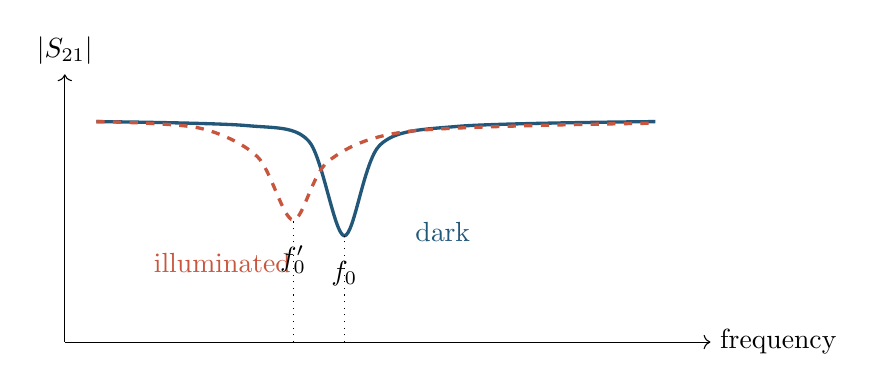
\begin{tikzpicture}[x=1cm,y=1cm]
\draw[->] (0,0)--(8.2,0) node[right]{frequency};
\draw[->] (0,0)--(0,3.4) node[above]{$|S_{21}|$};
\draw[very thick,KidBlue] plot[smooth] coordinates {(0.4,2.8)(2.3,2.75)(3.1,2.55)(3.55,1.35)(4.0,2.5)(5.0,2.74)(7.5,2.8)};
\draw[very thick,KidRed,dashed] plot[smooth] coordinates {(0.4,2.8)(1.7,2.72)(2.45,2.35)(2.9,1.55)(3.35,2.3)(4.4,2.68)(7.5,2.78)};
\node[KidBlue] at (4.8,1.4) {dark};
\node[KidRed] at (2.0,1.0) {illuminated};
\draw[dotted] (3.55,0)--(3.55,1.35) node[below,yshift=-2mm]{$f_0$};
\draw[dotted] (2.9,0)--(2.9,1.55) node[below,yshift=-2mm]{$f_0'$};
\end{tikzpicture}
\end{center}

\subsection{真正观测时：通常固定 probe tone，不需要不停扫频}
实际读出往往选取 $f_{\rm probe}\approx f_0$，持续测量一个复数：
\[
\boxed{S_{21}(t)=I(t)+jQ(t).}
\]
当谐振器因光照发生轻微移动时，固定 probe tone 在 resonance 曲线上的相对位置发生变化，因此 $I$ 和 $Q$ 随时间变化。

\begin{center}
\begin{tikzpicture}[scale=1.05]
\draw[->] (-2.6,0)--(2.8,0) node[right]{$I$};
\draw[->] (0,-2.3)--(0,2.5) node[above]{$Q$};
\draw[very thick,KidBlue] (0.35,0.05) circle (1.55);
\fill[KidBlue] (1.05,1.42) circle (2pt) node[above right]{dark operating point};
\fill[KidRed] (0.72,1.55) circle (2pt) node[above left]{illuminated};
\draw[-{Latex[length=2mm]},very thick,KidRed] (1.05,1.42)--(0.72,1.55);
\node[align=center] at (-1.4,-1.55) {扫频时形成\\近似 IQ 圆};
\end{tikzpicture}
\end{center}

这一步把 KID 与熟悉的数字接收机世界连接起来：最终进入 ADC/DSP 的不是“光子”本身，而是经过谐振器转导后的复基带响应。

\section{为什么读出微波不会自己把 Cooper pair 大量打碎？}
KID 中通常同时存在两种频率尺度：
\begin{align*}
\nu_{\rm signal} &\sim \text{几十到数百 GHz（毫米/亚毫米波）},\\
\nu_{\rm readout} &\sim \text{几百 MHz 到数 GHz（微波）}.
\end{align*}
设计上常希望
\[
h\nu_{\rm readout}<2\Delta,
\]
使单个 readout photon 的能量低于直接 pair-breaking threshold；与此同时
\[
h\nu_{\rm signal}>2\Delta,
\]
使目标光子能够被探测。

\begin{mistakebox}
“读出微波完全不影响超导态”也过于绝对。虽然单个低频 readout photon 通常不能直接 pair break，但过高读出功率仍会引起谐振器非线性、加热、准粒子分布变化等效应。因此实际系统存在最佳 readout power，而不是越大越好。
\end{mistakebox}

\section{LEKID 为什么尤其漂亮：同一块 meander 做两份工作}

\begin{center}
\begin{tikzpicture}[every node/.style={font=\small},arr/.style={-{Latex[length=2mm]},thick}]
\node[draw,rounded corners,fill=KidGold!18,minimum width=31mm,minimum height=12mm,align=center] (rad) {\SI{150}{GHz}\\入射辐射};
\node[draw,rounded corners,fill=KidTeal!10,minimum width=35mm,minimum height=15mm,align=center,right=14mm of rad] (mea) {meander inductor\\毫米波 absorber\\GHz kinetic inductor};
\node[draw,rounded corners,fill=KidBlue!8,minimum width=28mm,minimum height=15mm,align=center,right=14mm of mea] (idc) {IDC\\capacitor};
\node[draw,rounded corners,fill=KidGray,minimum width=31mm,minimum height=15mm,align=center,below=13mm of idc] (feed) {feedline\\GHz readout};
\draw[arr,KidGold!80!black] (rad)--node[above]{吸收} (mea);
\draw[arr,KidBlue] (mea)--node[above]{构成 LC} (idc);
\draw[arr,KidBlue] (feed)--node[right]{耦合} (idc);
\end{tikzpicture}
\end{center}

在 LEKID 中，lumped inductor 的 meander 往往同时承担：
\begin{enumerate}
  \item \textbf{毫米波/亚毫米波 absorber}：入射场在图形化薄膜中驱动高频电流并沉积能量；
  \item \textbf{GHz resonator 的电感}：其 $L_g+L_k$ 与 IDC 共同决定微波共振。
\end{enumerate}
因此，毫米波光学设计和 GHz 谐振器设计并不是两个独立问题；它们通过同一块超导薄膜耦合在一起。

\begin{projectbox}
对你的双偏振直接吸收 LEKID，今后每次看一个几何结构都可以问两个问题：\\
\textbf{光学问题：}它如何改变 \SI{150}{GHz} 场、电流分布、吸收和偏振选择性？\\
\textbf{读出问题：}它如何改变 $L_g$、$L_k$、$C$、$f_0$、$Q_i$、$Q_c$ 和可读出性？\\
这两个视角同时成立，才算真正理解 LEKID 几何设计。
\end{projectbox}

\section{把全章压缩成一张“因果链地图”}

\begin{center}
\begin{tikzpicture}[node distance=6mm, every node/.style={font=\small}, b/.style={draw,rounded corners,minimum width=52mm,minimum height=8mm,align=center}, a/.style={-{Latex[length=2mm]},thick,KidBlue}]
\node[b,fill=KidGold!18] (a) {$h\nu>2\Delta$\\信号光子被超导薄膜吸收};
\node[b,below=of a] (b) {Cooper pairs 被激发/破坏\\$N_{\qp}\uparrow$};
\node[b,below=of b] (c) {超导电磁响应改变\\$\sigma_1,\sigma_2$ 改变};
\node[b,below left=8mm and -6mm of c,fill=KidTeal!8] (d1) {$L_k\uparrow$\\总电感改变};
\node[b,below right=8mm and -6mm of c,fill=KidTeal!8] (d2) {微波耗散$\uparrow$\\$Q_i\downarrow$};
\node[b,below=18mm of c,fill=KidBlue!7] (e) {$f_0$ 和 resonance shape 改变};
\node[b,below=of e,fill=KidBlue!7] (f) {固定 probe tone 所见 $S_{21}$ 改变};
\node[b,below=of f,fill=KidGray] (g) {$I(t),Q(t)$\\数字后端估计光学信号};
\draw[a] (a)--(b);\draw[a] (b)--(c);\draw[a] (c)--(d1);\draw[a] (c)--(d2);\draw[a] (d1)--(e);\draw[a] (d2)--(e);\draw[a] (e)--(f);\draw[a] (f)--(g);
\end{tikzpicture}
\end{center}

\section{本章的“公式阶梯”}
第一遍学习只需要按下面顺序记忆，不需要同时掌握所有微观细节。

\begin{enumerate}
  \item 光子能量：
  \[
  E_\gamma=h\nu.
  \]
  \item Pair-breaking threshold：
  \[
  h\nu\ge2\Delta,
  \qquad
  \Delta(0)\approx1.764k_BT_c.
  \]
  \item 动能电感的核心比例关系：
  \[
  L_k\propto\frac1{n_s}.
  \]
  \item LC resonance：
  \[
  f_0=\frac1{2\pi\sqrt{LC}},\qquad L=L_g+L_k.
  \]
  \item 小信号频移：
  \[
  \frac{\delta f_0}{f_0}=-\frac{\alpha}{2}\frac{\delta L_k}{L_k}.
  \]
  \item 品质因数关系：
  \[
  \frac1{Q_r}=\frac1{Q_i}+\frac1{Q_c}.
  \]
  \item 实验读出量：
  \[
  S_{21}=I+jQ.
  \]
\end{enumerate}

\section{六个最容易形成的错误直觉}
\begin{enumerate}
  \item \textbf{“KID 直接测光子的电信号。”}\\
  不对。光先改变超导材料，再改变谐振器，最后才改变微波传输。
  \item \textbf{“只要 $h\nu>\Delta$ 就可以 pair break。”}\\
  基本阈值应是 $2\Delta$。
  \item \textbf{“Kinetic inductance 就是导线弯弯曲曲形成的电感。”}\\
  不对。弯曲几何主要影响 $L_g$；$L_k$ 来自超导载流子的惯性。
  \item \textbf{“光照只是让 resonance 左移。”}\\
  不完整。它通常也改变损耗和 $Q_i$。
  \item \textbf{“KID 工作时必须持续扫频。”}\\
  通常扫频用于定位与标定，真正时间序列读出常使用固定 probe tones。
  \item \textbf{“读出功率越大，SNR 一定越好。”}\\
  不对。过强驱动会进入非线性、加热或改变准粒子状态。
\end{enumerate}

\section{Day 1 的 3--4 小时任务}
如果今天只围绕这一章学习，建议按以下顺序：

\begin{tabularx}{\textwidth}{p{1.8cm} X X}
\toprule
时间 & 任务 & 完成标准 \\
\midrule
35 min & 手画“光子 $\rightarrow$ IQ”因果链，并写出每一箭头为什么成立 & 不看讲义可口述完整链条 \\
45 min & 独立重算 Al 在 $T_c=\SI{1.2}{K}$ 时的 $\Delta$、$2\Delta$ 和 $\nu_{\rm pb}$；再算 \SI{150}{GHz} 光子能量 & 能判断某个频率是否满足 pair-breaking 条件 \\
55 min & 从 $f_0=1/(2\pi\sqrt{LC})$ 推导小信号 $\delta f_0/f_0$，理解 $\alpha$ 的意义 & 推导不用背结果 \\
60 min & Python 画 notch resonator 的 $|S_{21}|$ 与 IQ 圆；令 $f_0$ 左移并比较固定 probe tone 的 $\Delta I,\Delta Q$ & 得到至少 3 张图 \\
30 min & 阅读 Day 2003 的摘要/图 1，并回看本章因果链 & 能指出论文实验的“被测量量”在哪里 \\
20 min & 闭卷回答本章 8 道题 & 至少 6 题能完整解释“为什么” \\
\bottomrule
\end{tabularx}

\section{闭卷理解检查}
\begin{checkpointbox}
不查资料，尝试回答：
\begin{enumerate}
  \item 为什么 pair-breaking threshold 是 $2\Delta$？
  \item 为什么 \SI{150}{GHz} 对 Al 是一个合理的 pair-breaking 频率，而 \SI{5}{GHz} 通常不是？
  \item $N_{\qp}$ 增加后，为什么不能只讨论 $L_k$ 而忽略 $Q_i$？
  \item $L_g$ 与 $L_k$ 的能量分别储存在什么地方？
  \item 为什么 $L_k$ 增加通常导致 $f_0$ 降低？
  \item 什么是 $Q_i,Q_c,Q_r$？
  \item 为什么实际观测可以固定 probe tone，而不必一直扫频？
  \item 用一句完整的话解释：LEKID 的 meander 为什么同时是 absorber 和 resonator inductor？
\end{enumerate}
\end{checkpointbox}

\section{本章结束后你应该拥有的“一个句子”}
如果只能保留一句话，应当是：

\begin{formula}
\centering
\Large
\textbf{KID 用高于能隙阈值的光改变超导薄膜的准粒子与复电导，再用高 $Q$ 微波谐振器把这种微小变化转成可精确测量的 $S_{21}=I+jQ$ 变化。}
\end{formula}

\chapter*{后续版本计划}
\addcontentsline{toc}{chapter}{后续版本计划}
\begin{itemize}
  \item v0.2：Cooper pair、BCS 能隙与热准粒子；
  \item v0.3：从牛顿/伦敦方程到 kinetic inductance，并引入 sheet inductance；
  \item v0.4：复电导与 Mattis--Bardeen 的器件化理解；
  \item v0.5：$Q_i/Q_c/Q_r$、notch resonator、IQ circle 与实际 fitting；
  \item v0.6：optical responsivity、quasiparticle lifetime、NEP 与噪声；
  \item v0.7：LEKID absorber / IDC / polarization / backshort 的电磁设计；
  \item v0.8：把上述理论逐项映射到当前双偏振 \SI{150}{GHz} LEKID 项目与 Sonnet/CST 验证矩阵。
\end{itemize}

\chapter*{建议参考资料}
\addcontentsline{toc}{chapter}{建议参考资料}
\begin{enumerate}
  \item P. K. Day et al., ``A broadband superconducting detector suitable for use in large arrays,'' \textit{Nature}, 425, 817--821 (2003).
  \item S. Doyle, \textit{Lumped Element Kinetic Inductance Detectors}, PhD thesis, Cardiff University (2008).
  \item J. Zmuidzinas, ``Superconducting Microresonators: Physics and Applications,'' \textit{Annual Review of Condensed Matter Physics}, 3, 169--214 (2012).
  \item J. Gao, \textit{The Physics of Superconducting Microwave Resonators}, PhD thesis, California Institute of Technology (2008).
\end{enumerate}

\end{document}
